% NeurIPS 2026 Paper Draft
% Title: Same Signal, Opposite Meaning: Why Adaptive Compute Fails Across Environments
% Template: NeurIPS 2026

\documentclass{article}
\PassOptionsToPackage{table}{xcolor}

% === NeurIPS 2026 Style ===
% Default option = anonymous double-blind submission with line numbers.
% For arXiv preprint: use [preprint]; for camera-ready: use [final].
\PassOptionsToPackage{authoryear,round}{natbib}
\usepackage{template/neurips_2026}
% Preserve ACL-style \cite -> \citep (parenthetical) to match existing manuscript text.
\let\citeOriginal\cite
\renewcommand{\cite}{\citep}
\usepackage{hyperref}
\usepackage{times}
\usepackage{latexsym}
\usepackage{amsmath}
\usepackage{amssymb}
\usepackage{amsthm}
\usepackage{graphicx}
\usepackage{wrapfig}
\usepackage{booktabs}
\usepackage{multirow}
\usepackage{enumitem}
\usepackage{xcolor}
\usepackage[most]{tcolorbox}
\tcbuselibrary{skins}
\usepackage{subcaption}
\usepackage{pifont}
\usepackage{float}
\usepackage{algorithm}
\usepackage{algpseudocode}
\DeclareMathOperator*{\argmin}{arg\,min}
\usepackage{tabularx}
\usepackage{booktabs}
\newcolumntype{L}{>{\raggedright\arraybackslash}X}
\newcolumntype{S}{>{\raggedright\arraybackslash\hsize=0.75\hsize}X}
\newcolumntype{B}{>{\raggedright\arraybackslash\hsize=1.0833\hsize}X}
\newcolumntype{N}{>{\raggedright\arraybackslash\hsize=0.6\hsize}X}
\newcolumntype{W}{>{\raggedright\arraybackslash\hsize=1.1333\hsize}X}
% === Theorem Environments ===
\newtheorem{proposition}{Proposition}
\newtheorem*{proposition*}{Proposition}
\newtheorem{definition}{Definition}

% === Shortcuts ===
\newcommand{\cmark}{\ding{51}}
\newcommand{\xmark}{\ding{55}}
\AtBeginDocument{%
  \setlength{\abovedisplayskip}{4pt}%
  \setlength{\belowdisplayskip}{4pt}%
  \setlength{\abovedisplayshortskip}{2pt}%
  \setlength{\belowdisplayshortskip}{2pt}%
}

\definecolor{PTGreen}{RGB}{92,134,110}
\definecolor{PTGreenDark}{RGB}{52,92,75}
\definecolor{PTLightGreen}{RGB}{242,250,245}
\definecolor{PTWhite}{RGB}{255,255,255}

\title{Same Signal, Opposite Meaning: Direction-Aware Adaptive Compute for LLM Agents}

% Anonymous submission for review
\author{Anonymous}

\begin{document}
\maketitle

% ============================================================
% ABSTRACT
% ============================================================
\begin{abstract}
Test-time compute improves decision quality for LLM agents, but deciding when it is beneficial remains unresolved. Existing gating methods rely on uncertainty signals, implicitly assuming a fixed relationship between signal value and compute benefit. We show that this assumption is incorrect. 
Across eight diverse agent environments and three model backbones, we find that the same signal value that predicts rollout benefit in one environment predicts rollout harm in another, indicating a reversal in the signal--utility relationship. 
We trace this to a conflation of two uncertainty sources, \emph{information poverty} and \emph{decision difficulty}, and formalize it via a two-source model grounded in Simpson's paradox, where subgroup-level trends reverse upon aggregation. We prove that direction discovery is a necessary condition for non-negative value of computation across environments. 
Motivated by this result, we propose EAAG (Environment-Aware Adaptive Gating), which learns environment-specific signal--utility relationships through direction discovery. Across eight environments, EAAG outperforms all fixed-direction baselines with zero additional per-step overhead, achieving adaptive gating behavior solely by learning signal direction. 
\end{abstract}


% ============================================================
% 1. INTRODUCTION
% ============================================================
\section{Introduction}
\label{sec:intro}

% --- Module 1: Why this problem matters (~45%) ---

Large language models (LLMs) have rapidly advanced across a wide
range of tasks, from question answering and code generation to web
navigation and embodied decision making~\cite{yao2023react,
shinn2023reflexion, zhou2024lats}. Yet, many tasks remain beyond the
reach of a single forward pass: complex reasoning, multi-step
planning, and open-ended exploration often require the model to
evaluate alternatives, verify intermediate results, or search over
candidate actions~\cite{yao2023tree, hao2023reasoning,
snell2024scaling}. This has motivated \emph{test-time compute}, where additional
computation at inference time improves decision quality. Across
multiple benchmarks, test-time optimization allows smaller models to
match or exceed the performance of larger ones at lower total
cost~\cite{snell2024scaling, wang2026flare}.

% While effective, test-time compute is expensive, incurring substantial per-step overhead (e.g., requiring multiple rollouts or candidate evaluations at each decision point)~\cite{yao2023tree, zhou2024lats}. As
% agents are deployed across diverse settings, applying this overhead
% uniformly becomes wasteful when only a fraction of steps benefit.
% This has motivated \emph{adaptive gating}: using uncertainty
% signals to decide \emph{when} extra compute is worthwhile.
% Prior work explores diverse mechanisms, including entropy thresholding~\cite{seag2025, cats2025, corefine2026}, calibrated confidence~\cite{s1_2025, han2025tokenbudget}, vote disagreement~\cite{catts2026}, and reinforcement learning~\cite{adaptthink2025, thinkless2025}. Across these mechanisms, adaptive gating consistently reduces cost while preserving or improving task performance within each method's evaluation setting.
While effective, test-time compute is expensive, incurring substantial per-step overhead (e.g., requiring multiple rollouts or candidate evaluations at each decision point)~\cite{yao2023tree, zhou2024lats}. As
agents are deployed across diverse settings, applying this overhead
uniformly becomes wasteful when only a fraction of steps benefit.
This has motivated \emph{adaptive gating}: using uncertainty
signals to decide \emph{when} extra compute is worthwhile.
Prior work explores diverse mechanisms, including entropy thresholding~\cite{seag2025, cats2025, corefine2026}, calibrated confidence~\cite{s1_2025, han2025tokenbudget}, vote disagreement~\cite{catts2026}, and learned difficulty estimators based on hidden states or reinforcement learning~\cite{diffadapt2025, zhu2025llmalreadyknows, adaptthink2025, thinkless2025}. Across these mechanisms, adaptive gating consistently reduces cost while preserving or improving task performance within each method's evaluation setting.

% Yet these gains often fail to transfer: methods calibrated for one task type frequently fail when applied to others~\cite{tao2025revisiting,
% heo2025llmuncertainty}. Vote-based
% gating designed for web agents degrades on fact-verification tasks;
% calibration-based methods that perform well on QA degrade in code
% generation. In several cases, adaptive gating \emph{actively
% harms} performance compared to never invoking the optimizer. This
% raises a central question: \emph{do uncertainty signals have a
% universal relationship with compute value, or does this relationship
% depend on the environment?}
However, this consensus rests on a narrow empirical base. The
fixed-direction assumption holds well in the settings where these
methods have been developed and evaluated, predominantly homogeneous
reasoning benchmarks where signal direction is consistent by
construction. Whether it transfers to heterogeneous agent
environments is an open question prior work has not directly
addressed, and we show that it does not: the relationship between
uncertainty and compute value can reverse direction across
environments, and adaptive gating can actively underperform never
invoking the optimizer. This raises a central question:
\emph{what determines the relationship between uncertainty signals
and the value of computation, and can this relationship be learned
in a way that generalizes across environments?}

% --- Module 2: Our finding + diagnosis (~30%) ---

% We conduct systematic measurement across eight agent environments spanning QA~\cite{yang2018hotpotqa}, code generation~\cite{hendrycks2021apps}, web navigation~\cite{yao2022webshop}, fact verification~\cite{thorne2018fever}, and text games~\cite{jansen2023twexpress}, using three model backbones. The signal–utility direction \emph{reverses} across environments: the same signal that predicts rollout benefit in code generation predicts rollout harm in fact verification, and can further reverse across model backbones within the same environment. Beyond direction, the most informative signal itself varies across environments, with structural features dominating in some while entropy carries no information.
We answer this through systematic measurement across six agent environments spanning QA~\cite{yang2018hotpotqa}, code
generation~\cite{hendrycks2021apps}, web navigation~\cite{yao2022webshop}, fact verification~\cite{thorne2018fever}, text games~\cite{jansen2023twexpress}, and crafting planning, using three model backbones. The signal--utility relationship reverses direction across environments:
the same signal that predicts rollout benefit in code generation predicts rollout harm in fact verification, and can further reverse
across model backbones within the same environment. Moreover, the most informative signal itself varies across environments, with
structural features dominating in some settings while entropy carries little or no information in others.
 
% We trace this reversal to a conflation of two uncertainty sources.
% \emph{Information poverty} arises when the agent lacks sufficient
% data; here rollouts from the same model cannot compensate, and high
% entropy predicts rollout harm. \emph{Decision difficulty} arises
% when the agent faces multiple viable paths; here rollouts explore
% alternatives productively, and high entropy predicts rollout benefit.
% Environments differ in the proportion of these two state types,
% causing the same signal to carry opposite meaning. This is an
% instance of Simpson's paradox~\cite{simpson1951interpretation,kdd2023simpson} in the signal--utility space. We prove
% that this has a sharp consequence: no fixed-direction gate can
% guarantee non-negative value of computation across environments with
% opposing directions (Proposition~\ref{prop:necessity}). Once the
% direction is wrong, more precise calibration makes performance
% \emph{worse}, because the gate more precisely targets harmful states.
We trace this reversal to a conflation of two distinct sources of uncertainty. \emph{Information poverty} (Type~I) arises when the
agent lacks sufficient information; rollouts from the same model cannot compensate, and high uncertainty predicts \emph{negative}
value of computation. In contrast, \emph{decision difficulty} (Type~D) arises when multiple viable options exist; additional
computation helps explore alternatives, and high uncertainty predicts \emph{positive} value. Code generation often involves
multiple valid implementations (Type~D), while fact verification may lack sufficient evidence altogether (Type~I). Because
environments differ in their mixture of these two state types, the same uncertainty signal carries opposite meanings depending on
which source dominates, a phenomenon closely related to Simpson's paradox~\cite{simpson1951interpretation,kdd2023simpson}. The
consequence is sharp: no fixed-direction gating strategy can avoid net-harmful gating across environments with opposing signal
directions (Proposition~\ref{prop:necessity}), and once the direction is misaligned, improved calibration can \emph{worsen} performance by more precisely selecting harmful states.

% --- Module 3: Method + contributions (~25%) ---

% Motivated by this analysis, we propose \textbf{EAAG}
% (\textbf{E}nvironment-\textbf{A}ware \textbf{A}daptive
% \textbf{G}ating), which discovers environment-specific gating
% patterns through randomized \emph{exploration}, LLM-based
% \emph{reasoning} about exploration data, and sparse
% \emph{learning} of signal direction and importance.
% Since direction is the primary determinant of gate quality, not
% model capacity, EAAG pairs a rich discovery process with a
% deliberately simple gate that adds zero per-step deployment cost.
% EAAG outperforms all fixed-direction baselines across eight
% environments and three LLM backbones.
Motivated by this analysis, we propose \textbf{EAAG} (\textbf{E}nvironment-\textbf{A}ware \textbf{A}daptive \textbf{G}ating), a deliberately minimal method that learns environment-specific signal–utility relationships from interaction data. Since the primary challenge is identifying signal direction rather than modeling capacity, EAAG's contribution is not a new gate architecture but a pipeline that reduces the adaptive-gating problem to a form where a standard sparse linear classifier suffices, adding zero per-step cost at deployment. Across six environments and three LLM backbones, EAAG outperforms all fixed-direction baselines.
%Importantly, since signal direction cannot be inferred from uncertainty alone and varies across environments, it must be discovered through interaction data, rather than assumed or calibrated from static signals.

Taken together, these results point to a more fundamental
observation: uncertainty signals like token entropy are not
sufficient statistics for the value of computation, because their
meaning depends on a latent state property that the signal alone
cannot identify. Direction discovery is the minimal mechanism that
closes this gap.

Our main contributions are as follows:
\begin{itemize}[leftmargin=*,nosep]
\item \textbf{A structural limitation of uncertainty-based gating.}
We show that uncertainty signals are not sufficient statistics for
the value of computation: their meaning depends on a latent state
type, and as a consequence no fixed-direction gate can be
universally correct.

\item \textbf{Empirical finding.} We demonstrate systematic reversal of signal--utility direction across environments and model backbones, and show that the most informative signals vary across settings.

\item \textbf{Adaptive gating method.} We propose EAAG, which learns signal direction per environment instead of assuming it, outperforming all fixed-direction baselines across six environments with zero deployment overhead.
\end{itemize}


% ============================================================
% 2. RELATED WORK
% ============================================================
\section{Related Work}
\label{sec:related}

\paragraph{Adaptive test-time compute.}
Adaptive gating methods reduce the overhead of test-time
optimization by invoking it only when needed. In the
\emph{reasoning} setting, signal-based methods use token-level
confidence or entropy to decide when to extend
thinking~\citep{seag2025, cats2025, corefine2026,
thinkjustenough2025, s1_2025, han2025tokenbudget}. RL-based methods
learn think/no-think policies through reinforcement
learning~\citep{adaptthink2025, thinkless2025, aggarwal2025l1},
though these require per-environment training and provide no
interpretable direction signal. Hidden-state probing
methods~\citep{diffadapt2025, zhu2025llmalreadyknows} train
lightweight classifiers on internal representations to estimate task
difficulty, assuming a universal difficulty-to-compute mapping.
In the \emph{agent} setting, vote-based
methods~\citep{catts2026} sample multiple candidate actions and
trigger evaluation when disagreement is high, and
\citet{paglieri2025learning} learn when to invoke a planner at the
episode level. The vast majority of adaptive compute research
operates on homogeneous reasoning benchmarks (MATH, GSM8K, GPQA),
where signal direction happens to be consistent across tasks. Our
work is the first to systematically study signal semantics across
heterogeneous \emph{agent} environments, where we find that the
direction reverses. A detailed per-method comparison is provided in
Appendix~\ref{app:related}.

\paragraph{Test-time scaling and search.}
Test-time scaling~\citep{snell2024scaling} studies compute-optimal
allocation at the problem level, showing that adaptive allocation
outperforms uniform allocation by up to 4$\times$ in efficiency.
This line of work focuses on \emph{how much} compute to allocate
given a fixed difficulty signal, whereas we question the signal
itself. Search methods such as Tree of
Thoughts~\citep{yao2023tree}, LATS~\citep{zhou2024lats},
RAP~\citep{hao2023reasoning}, and FLARE~\citep{wang2026flare}
improve the quality of the search process through tree search,
value propagation, and lookahead evaluation. These are complementary
to our work: they improve \emph{what} the optimizer does, while we
control \emph{when} to invoke it. Our gating framework can be
composed with any such optimizer.

\paragraph{Uncertainty estimation and metareasoning.}
Recent work on LLM uncertainty~\citep{tao2025revisiting,
heo2025llmuncertainty} observes that calibration quality varies
substantially across task types, providing converging evidence that
uncertainty semantics are domain-dependent. \citet{yadkori2024believe}
propose decoupling epistemic and aleatoric uncertainty in LLM
outputs, a distinction conceptually related to our Type~I/Type~D
decomposition. From a decision-theoretic perspective, rational
metareasoning~\citep{russell1991right, desabbata2024metareasoning}
formalizes the value of computation (VOC) as a guide for allocating
cognitive resources. Our work extends this framework by showing
that VOC can be \emph{negative} in the agent setting when the
evaluator and executor are the same model, and that direction
discovery is a necessary condition for non-negative VOC across
environments.


% ============================================================
% 3. WHY FIXED-DIRECTION GATING FAILS
% ============================================================
\section{Why Fixed-Direction Gating Fails}
\label{sec:signal-landscape}
\begin{table}[!t]
\caption{Signal--utility correlations across 6 environments and
3 backbones. $\rho$: Spearman correlation of token entropy with
optimizer utility $U$. $^*$: significant at $p{<}0.05$.
Direction varies across \emph{both} environments and model
backbones.}
\vspace{-0.1in}
\label{tab:signal-discovery}
\centering\small
\setlength{\tabcolsep}{4pt}
\begin{tabular}{lcccc}
\toprule
Environment & Qwen3 & Phi-3.5 & Llama-3.1 & Cons. \\
\midrule
HotpotQA   & $-$0.327$^*$ & $+$0.184$^*$ & $-$0.346$^*$ & \xmark \\
WebShop    & $+$0.133$^*$ & $+$0.335$^*$ & $+$0.287$^*$ & \cmark \\
FEVER      & $-$0.119$^*$ & $-$0.156$^*$ & $+$0.428$^*$ & \xmark \\
APPS       & $+$0.317$^*$ & $-$0.024     & $-$0.249$^*$ & \xmark \\
TWExpress  & $-$0.290$^*$ & $+$0.000     & $+$0.000     & --- \\
Plancraft  & $-$0.016     & $+$0.000     & $-$0.176$^*$ & --- \\
\bottomrule
\end{tabular}
\end{table}

We first formalize the adaptive gating problem, then measure
signal--utility correlations across diverse environments to test
the fixed-direction assumption.

We study LLM-based agents in multi-step interactive environments.
At each step $t$, the agent observes state $s_t$, selects action
$a_t$, and transitions to $s_{t+1}$. An environment-specific
\emph{test-time optimizer} $T$ (e.g., rollout evaluation, $K$-variant
sampling) can be invoked at any step to potentially improve action
quality. Let $\sigma(s)$ denote the uncertainty signal at state $s$
(e.g., token entropy of the next-token distribution). We define
the \emph{optimizer utility} as:
\begin{equation}
  U(T, s) = \mathbb{E}[R(\tau) \mid a{=}T(s)]
           - \mathbb{E}[R(\tau) \mid a{=}\pi(s)]
  \label{eq:utility}
\end{equation}
where $R(\tau)$ is the episode return. $U > 0$ indicates the
optimizer improves the outcome; $U \leq 0$ indicates it is wasteful
or harmful. The \emph{adaptive gating problem} is to learn a gate
$g: \mathcal{S} \to \{0, 1\}$ that triggers $T$ only when $U > 0$.

\subsection{Signal--Utility Direction Reverses Across Environments
            and Backbones}
\label{sec:empirical-landscape}

\textbf{The signal--utility direction is not fixed.}
Table~\ref{tab:signal-discovery} reports Spearman correlations
between token entropy and optimizer utility across 6 environments
<<<<<<< HEAD
and 3 model backbones~\cite{DBLP:journals/corr/abs-2505-09388,DBLP:journals/corr/abs-2407-21783,DBLP:journals/corr/abs-2404-14219}. Two patterns stand out, and the more striking one is the harder to explain. First, \emph{the same signal in the same environment can reverse across
backbones}: in 3 out of 4 environments with multiple significant
correlations, the backbones disagree on the sign of $\rho$. The
most extreme case is FEVER, which flips from $\rho{=}{-}0.156$ on
Phi-3.5 to $\rho{=}{+}0.428$ on Llama-3.1---a sign change driven
=======
and 3 model backbones~\cite{DBLP:journals/corr/abs-2505-09388,DBLP:journals/corr/abs-2407-21783,DBLP:journals/corr/abs-2404-14219}. First, \emph{the same signal in the same environment can reverse across
backbones}: among environments with at least two significant nonzero correlations, sign disagreement across backbones is common. The most extreme case is FEVER, which flips from $\rho{=}{-}0.156$ on Phi-3.5 to $\rho{=}{+}0.428$ on Llama-3.1, a sign change driven
>>>>>>> 1bf5b0e2c05afb339eb3e76f610bbf4ff034c5a3
entirely by the choice of LLM, with the task held fixed. The
signal's semantics are therefore not a property of the
environment alone, but of how the agent's prior knowledge
interacts with it. Second, \emph{even within a single backbone,
the direction also varies across environments}: on Qwen3, entropy
is negatively correlated with utility in information-seeking
environments (FEVER, HotpotQA, TWExpress) but positively in code
generation (APPS) and web navigation (WebShop), with near-zero
correlation in weak-signal environments (Plancraft). Crucially,
this direction mismatch is not benign: as
Section~\ref{sec:main-results} will show, gates that assume the
wrong direction systematically fall \emph{below} the no-trigger
baseline, making them strictly worse than doing nothing in
mismatched (environment, backbone) pairs.
<<<<<<< HEAD

\paragraph{Implication: $\sigma$ is not a sufficient statistic
for VOC.}
The reversal in Table~\ref{tab:signal-discovery} is not just
``fixed-direction gating fails''---it is the empirical signature
of a stronger structural fact. Across (environment, backbone)
settings, two states with identical $\sigma$ values can have
opposite-sign value of computation, depending on whether the
agent is in an information-poor or decision-difficult state
(\S\ref{sec:toy-model}). Hence $\sigma$ is not a sufficient
statistic for $\mathrm{VOC}$, and \emph{no} policy of the form
$g(\sigma(s))$---monotone or otherwise, calibrated or
not---can deliver non-negative value of computation across
heterogeneous settings (Proposition~\ref{prop:necessity}, proof
in Appendix~\ref{app:proof-necessity}). Fixed-direction gating
is the strict-monotone special case; the underlying obstruction
is a property of the signal itself, not of how the gate
post-processes it. Recovering sufficiency therefore requires
augmenting $\sigma$ with auxiliary features that distinguish
the two state types---a requirement that directly motivates
the multi-feature design of \S\ref{sec:method}.

\paragraph{A diagnostic for practitioners.}
The reversal test of Table~\ref{tab:signal-discovery} is itself
the leave-behind tool of this paper: collecting a few hundred
signal-agnostic $(s, U)$ pairs and reporting the Spearman
correlation $\rho(\sigma, U)$ together with its bootstrap
confidence interval is sufficient to decide whether a fixed
direction is safe for a given (environment, backbone) deployment.
A confidence interval that crosses zero, or two settings that
disagree on sign, indicates that any uncertainty-thresholding
gate will eventually fall below never-gating; a stable
single-sign correlation indicates that fixed-direction gating is
safe and direction learning is unnecessary. We apply this
diagnostic throughout, and recommend it as a standalone check
independent of the specific learning procedure adopted.
=======
>>>>>>> 1bf5b0e2c05afb339eb3e76f610bbf4ff034c5a3

\textbf{Signal identity also varies across environments.}
Beyond direction, the most informative signal itself differs
across environments: \texttt{step\_count} dominates in most
settings, but WebShop relies on \texttt{num\_available\_actions}
instead (Appendix~\ref{app:feature-selection}). No single signal
is reliably informative; multi-signal gates substantially
outperform single-feature gates
(Appendix~\ref{app:auc}). These observations suggest that
uncertainty is entangled with latent state structure that varies
across (environment, backbone) pairs. We formalize this intuition
next.

\subsection{Why Does Direction Reverse? A Two-Source Model}
\label{sec:toy-model}

The findings above establish that fixed-direction gating fails; we
<<<<<<< HEAD
now ask \emph{why}. We trace direction reversal to two coexisting
state types with opposite signal--utility relationships.

\paragraph{Intuition.}
Consider two agents that both hesitate (high entropy) at a
decision point. A coding agent hesitates because multiple valid
implementations exist; rollouts explore these alternatives
productively, so high entropy positively predicts rollout utility
(Type~D). A fact-verification agent hesitates because the
retrieved evidence is ambiguous; rollouts from the same model
draw observations from the \emph{same} information-bounded
environment, so they cannot synthesize evidence the environment
did not provide, and high entropy instead predicts rollout
\emph{futility} (Type~I). The same numerical signal carries
opposite meaning because the \emph{source} of uncertainty
differs.
=======
now ask \emph{why}. We model direction reversal as arising from two coexisting state types with opposite signal--utility relationships. As discussed in \S\ref{sec:intro}, high entropy carries opposite
meaning depending on whether the agent lacks information
(Type~I, where rollouts cannot help) or faces multiple viable
options (Type~D, where rollouts productively explore
alternatives).
>>>>>>> 1bf5b0e2c05afb339eb3e76f610bbf4ff034c5a3

\paragraph{Model.}
We model direction reversal as arising from two state types at each
decision step:
\begin{itemize}[leftmargin=*,nosep]
\item \textbf{Type~I (information poverty):} Utility is
  \emph{negatively} related to entropy:
  $U_I(s) \sim -\alpha H(s) + \varepsilon_I$, $\alpha > 0$.
\item \textbf{Type~D (decision difficulty):} Utility is
  \emph{positively} related to entropy:
  $U_D(s) \sim +\beta H(s) + \varepsilon_D$, $\beta > 0$.
\end{itemize}
Let $p_I(\mathcal{E})$ denote the fraction of Type~I states in
environment $\mathcal{E}$. The marginal correlation becomes
\begin{equation}
  \rho(\mathcal{E}) \;\approx\;
  \beta - (\alpha + \beta)\,p_I(\mathcal{E}),
  \label{eq:direction}
\end{equation}
which reverses sign at the critical threshold
$p_I^* = \beta/(\alpha+\beta)$. Environments with
$p_I > p_I^*$ exhibit negative $\rho$ (Type~I dominated); those
with $p_I < p_I^*$ exhibit positive $\rho$ (Type~D dominated);
near $p_I^*$, the two effects cancel and entropy carries
<<<<<<< HEAD
negligible signal. This prediction is consistent with the observed
Qwen3 pattern in Table~\ref{tab:signal-discovery}: search-based QA
(FEVER, HotpotQA, TWExpress) shows negative $\rho$, code
generation (APPS) shows positive $\rho$, and weak-signal
environments (Plancraft) cluster near zero.

\paragraph{Backbone-level reversal is a prediction, not an
anomaly.} A subtlety is essential here: $p_I$ is not a property
of the environment alone. A state is information-poor only
relative to what the agent already encodes; the same observation
can be Type~I for one model and Type~D for another. The model
backbone therefore enters the mixture directly, and the effective
$p_I$ is indexed by the (environment, backbone) pair. Read this
way, the backbone-level sign flips of
Table~\ref{tab:signal-discovery}---most extreme on FEVER between
Phi-3.5 and Llama-3.1---are exactly what the model predicts:
backbone changes shift $p_I$, and when they cross $p_I^*$, $\rho$
flips. Far from contradicting the two-source view, backbone
reversal becomes one of its predictions
(Appendix~\ref{app:multi-backbone}).
=======
negligible signal. This expression captures the sign-level
dependence of the marginal trend on the mixture proportion under
a simplified linear model; it is not intended as a precise
estimator of Spearman $\rho$. The prediction is consistent with
the observed Qwen3 pattern in Table~\ref{tab:signal-discovery}:
search-based QA (FEVER, HotpotQA, TWExpress) shows negative
$\rho$, code generation (APPS) shows positive $\rho$, and
weak-signal environments (Plancraft) cluster near zero.

\paragraph{Backbone-level reversal is a prediction, not an
anomaly.} $p_I$ is not a property of the environment alone. A
state is information-poor only relative to what the agent already
encodes; the same observation can be Type~I for one model and
Type~D for another. The model backbone therefore enters the
mixture directly, and the effective $p_I$ is indexed by the
(environment, backbone) pair. The backbone-level sign flips of
Table~\ref{tab:signal-discovery}, most extreme on FEVER between
Phi-3.5 and Llama-3.1, are exactly what the model predicts:
backbone changes shift $p_I$, and when they cross $p_I^*$, $\rho$
flips (Appendix~\ref{app:multi-backbone}).
>>>>>>> 1bf5b0e2c05afb339eb3e76f610bbf4ff034c5a3

\paragraph{Theoretical grounding.}
This direction reversal is a special case of Simpson's
paradox~\cite{simpson1951interpretation,DBLP:books/acm/22/Pearl22n}:
aggregating subpopulations with opposing within-group trends
reverses the aggregate correlation. Our decomposition adapts the
epistemic/aleatoric distinction~\cite{der2009aleatory} to the
meta-decision setting: Type~I states exhibit epistemic-like
uncertainty (information deficit), while Type~D states exhibit
aleatoric-like diversity (multiple viable paths). We treat this
two-source decomposition as a \emph{minimal falsifiable} model
rather than a post-hoc explanation: in
Section~\ref{sec:theory-verification} we derive three predictions
from it (temporal dynamics, cross-environment consistency, and
signal identity alignment) and verify each on held-out data.

<<<<<<< HEAD
The decomposition also makes the insufficiency claim of
\S\ref{sec:empirical-landscape} precise. Since the latent type
$\tau(s) \in \{I, D\}$ governs the sign of $\mathrm{VOC}(s)$
but is not measurable from $\sigma(s)$ alone, no function of
$\sigma$ can recover $\tau$, and therefore no function of
$\sigma$ can recover the sign of $\mathrm{VOC}$. The
information-theoretic content of the reversal is exactly this
non-identifiability of $\tau$ from $\sigma$.

% §3.3 (Necessity of Direction Discovery) folded into §3.1
% "Implication." paragraph above; full proposition and proof are
% deferred to Appendix~\ref{app:proof-necessity}.
=======
\paragraph{Implication.}
Under this decomposition, $\sigma$ is not a sufficient statistic
for $\mathrm{VOC}$: two states with identical $\sigma$ but
opposite latent types have opposite-sign utility. No policy of the
form $g(\sigma(s))$ can therefore deliver non-negative value across
heterogeneous settings, and uncertainty-only fixed-direction gates
empirically fail across our six environments
(Proposition~\ref{prop:necessity}, proof in
Appendix~\ref{app:proof-necessity}). Recovering sufficiency
requires augmenting $\sigma$ with features that distinguish the two
state types, directly motivating the multi-feature design of
\S\ref{sec:method}.

% \paragraph{A diagnostic for practitioners.}
% Collecting a few hundred signal-agnostic $(s, U)$ pairs and
% reporting $\rho(\sigma, U)$ with its bootstrap confidence interval
% is sufficient to decide whether a fixed direction is safe for a
% given deployment. A confidence interval that crosses zero
% indicates that fixed-direction gating is unreliable; a stable
% single-sign correlation indicates it is safe.
>>>>>>> 1bf5b0e2c05afb339eb3e76f610bbf4ff034c5a3


% ============================================================
% 4. METHOD: DIAL
% ============================================================
\begin{figure*}[t]
	\centering
	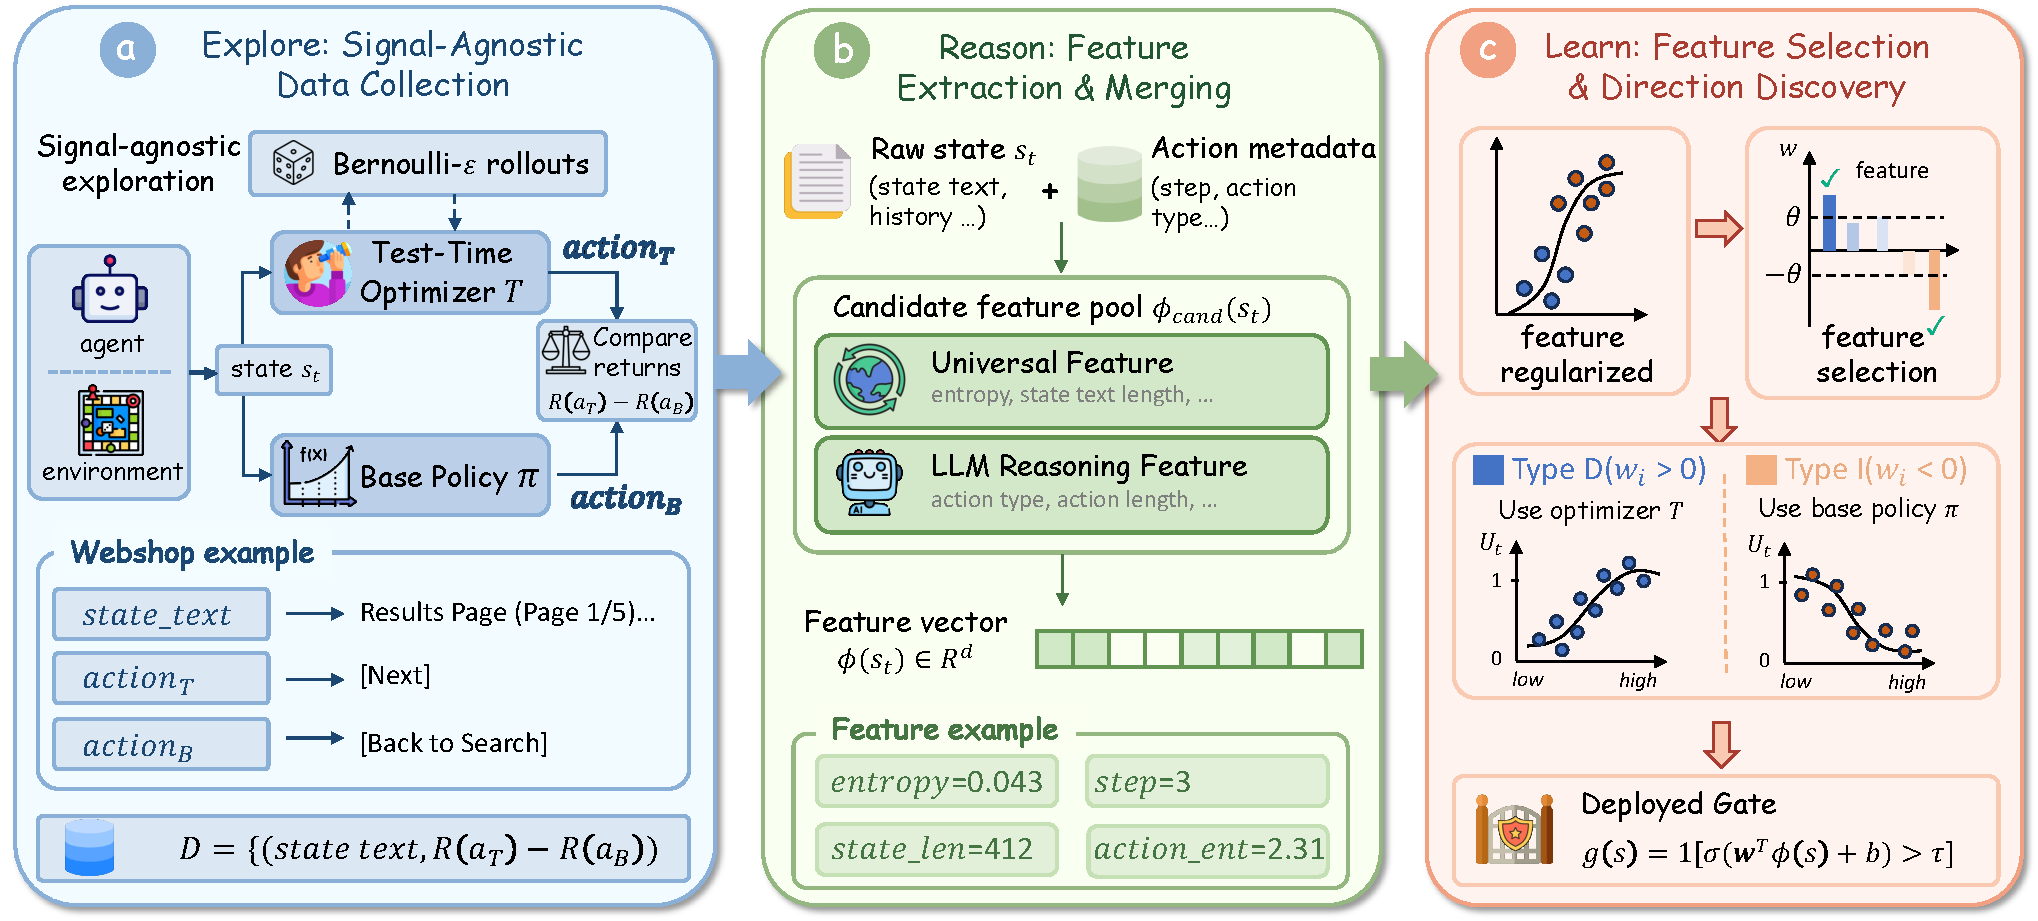
\includegraphics[width=\textwidth]{figures/dial_pipeline4.pdf} 
    \vspace{-0.2in}
	\caption{\textbf{The DIAL pipeline.}
		\textbf{(a) Explore}: collect signal-agnostic $(s, U)$ pairs via Bernoulli-$\varepsilon$ rollouts.
		\textbf{(b) Reason}: build a candidate feature pool $\phi(s)$ from universal metrics combined with LLM-proposed task-specific features.
		\textbf{(c) Learn}: fit an $\ell_1$-regularized logistic gate, whose signed weights jointly perform feature selection and recover per-environment direction (Type~D: $w_i{>}0$; Type~I: $w_i{<}0$).}
	\label{fig:method_overview}
\end{figure*}
\vspace{-0.1in}
\section{Direction-Informed Adaptive Learning}
\label{sec:method}
\vspace{-0.1in}
DIAL reframes gating from difficulty estimation to intervention-utility estimation: it trains on counterfactual optimizer utility rather than difficulty or correctness proxies, and uses signal-agnostic exploration so that the learned gate can discover when each feature indicates positive or negative rollout value instead of inheriting a fixed direction from the data collection rule.
The analysis in \S\ref{sec:signal-landscape} implies three constraints for any cross-setting adaptive gate. It must (i) \emph{discover} the signal-utility direction per (environment, backbone) pair rather than hardcoding it; (ii) draw from a \emph{multi-signal feature pool} that approximates the latent state type $\tau(s)$, since no single signal is reliable across settings; and (iii) collect training data \emph{without conditioning on} the very signal whose direction is unknown, otherwise the data is biased toward the prior assumption. DIAL satisfies these three constraints in three stages (Fig.~\ref{fig:method_overview}): randomized exploration (\S\ref{sec:explore}), feature construction (\S\ref{sec:reason}), and sparse gate fitting (\S\ref{sec:learn}).

\vspace{-0.1in}
\subsection{Explore: Signal-Agnostic Data Collection}
\label{sec:explore}
\vspace{-0.05in}
The exploration stage collects the $(s, U)$ pairs used to fit the gate, under one central constraint: the collection policy must remain independent of any signal whose semantics we are trying to learn. A gate trained on uncertainty-triggered states would systematically under-sample the states that determine $\rho$'s sign, baking the prior assumption into the training data instead of testing it.

DIAL therefore uses the simplest policy consistent with this constraint. At each step~$t$ in episode~$i$, a uniform random coin flip with probability $\varepsilon_{\text{explore}}$ determines whether to trigger the optimizer~$T$ ($z_t^{(i)}{=}1$) or use the base action ($z_t^{(i)}{=}0$). For each step with $z_t^{(i)}{=}1$, we estimate utility by paired counterfactual rollouts from the same state snapshot: we fork the environment, execute both the optimizer's chosen action and the base action via truncated rollouts of horizon $H$, and record which yields a higher return. We set $U_t^{(i)} = 1$ if the optimizer's action wins, and $0$ otherwise. The Bernoulli trigger eliminates selection bias, and the paired design eliminates baseline bias; the remaining approximation is the truncation horizon $H$. Aggregating across $N_{\text{explore}}$ episodes yields the dataset:
\begin{equation}
  \mathcal{D} = \bigl\{
    \bigl(\phi(s_t^{(i)}),\; U_t^{(i)}\bigr)
    : z_t^{(i)} = 1
  \bigr\}_{t, i},
  \label{eq:dataset}
\end{equation}
where $\phi(s)$ is the feature vector. Per-environment estimation details are in Appendix~\ref{app:environment}.

\vspace{-0.1in}
\subsection{Reason: Feature Construction}
\label{sec:reason}
\vspace{-0.05in}
The next stage builds the candidate feature pool $\phi_{\text{cand}}(s)$. This pool must be rich enough to capture each environment's informative signals, but not so environment-specific that deployment requires manual engineering per task.

DIAL's candidate pool combines two layers. The first is a small set of universal features defined identically across environments: \texttt{step\_count}, \texttt{token\_entropy}, \texttt{evidence\_count}, \texttt{num\_available\_actions}, and \texttt{is\_finish} (definitions in Table~\ref{tab:universal-features}). Signals an environment does not naturally expose (e.g., \texttt{evidence\_count} outside QA-style tasks) default to zero, requiring no per-environment engineering. The second is an LLM-generated layer: an LLM receives a summary of $\mathcal{D}$ and proposes task-specific feature hypotheses $\phi_{\text{LLM}}(s)$, forming $\phi_{\text{cand}}(s) = \phi_{\text{univ}}(s) \cup \phi_{\text{LLM}}(s)$. The $\ell_1$ penalty in the next stage automatically discards uninformative proposals, so the LLM layer can propose freely without degrading gate quality. We show in \S\ref{sec:ablation} that the universal pool alone already outperforms all fixed-direction baselines, and the LLM layer adds further gains in environments where universal features are inadequate. We provide the prompt template and per-environment ablation in Appendix~\ref{app:llm-feature-layer} and Appendix~\ref{app:llm-features}.

\vspace{-0.1in}
\subsection{Learn: Sparse Linear Gate}
\label{sec:learn}
\vspace{-0.05in}

Given $\mathcal{D}$ and $\phi_{\text{cand}}$, DIAL fits an $\ell_1$-regularized logistic regression with the binary cross-entropy loss, where the regularization strength $\lambda$ controls sparsity over $\phi_{\text{cand}}$ so that uninformative features drop out. Let $(\mathbf{w}^*, b^*)$ denote the fitted weights and bias. The deployed gate is
\begin{equation}
  g(s) = \mathbf{1}\!\left[\mathrm{sigmoid}(\mathbf{w}^{*\top} \phi(s) + b^*) > \tau\right],
  \label{eq:gate}
\end{equation}
with threshold $\tau$ set by cross-validation on $\mathcal{D}$. At deployment, the gate requires only a feature evaluation and a single sigmoid: no extra LLM calls, no $K$-way voting, no calibration query. This zero-overhead deployment contrasts with prior gating methods that incur per-step costs (e.g., CATTS triggers $K{=}5$ forward passes per step, AUQ issues a confidence query every step).

\textbf{Signed weights as a diagnostic.}
The $\ell_1$ penalty simultaneously performs feature selection and direction discovery. The sign of each fitted weight provides an interpretable per-environment estimate of how the feature relates to optimizer utility: $w_i > 0$ indicates that feature~$i$ behaves as a decision-difficulty proxy in this setting, where larger values increase expected rollout value; $w_i < 0$ indicates an intervention-unsuitability proxy, where larger values mark states in which rollouts are less likely to help; and $w_i \approx 0$ indicates that the feature is uninformative. The complete pipeline, including online adaptation for drifting environments and detailed cost accounting, is in Appendix~\ref{app:dial-details}.

% ============================================================
% 5. EXPERIMENTS
% ============================================================
\section{Experiments}
\label{sec:experiments}

\subsection{Experimental Setup}
\label{sec:setup}

We evaluate EAAG along three axes: (1)~Does environment-aware gating
Pareto-dominate fixed-direction baselines across diverse environments?
(\S\ref{sec:main-results}) (2)~Which components (direction learning,
multi-signal features, LLM reasoning) drive the gains?
(\S\ref{sec:ablation}) (3)~Do the Two-Source Model's predictions
hold empirically? (\S\ref{sec:theory-verification})

\paragraph{Environments.} We evaluate on 8 environments spanning QA,
code generation, web navigation, fact verification, text games, and
crafting planning (Table~\ref{tab:env-setup}): HotpotQA,
APPS Intro, WebShop, FEVER, TWExpress, Plancraft, APPS Interview,
and CRUXEval. These environments are selected to cover the full
range of the Two-Source Model, from pure Type~I (FEVER) through
mixed ($\approx p_I^*$, APPS Intro) to Type~D (APPS Interview),
including extreme rollout properties (TWExpress: rollout-safe;
Plancraft: rollout-harmful).

\paragraph{Baselines.} All methods share the same agent and
optimizer $T$; we compare only the gate decision.
(1)~\emph{Bounds}: base\_only, always\_trigger, oracle.
(2)~\emph{Fixed-direction CB}: CaTS, SEAG, CoRefine, CATTS, AUQ,
s1\_budget, all assuming high uncertainty $\to$ trigger.
(3)~\emph{Ablation}: BSW (intentionally reversed direction).
(4)~\emph{Ours}: EAAG.
Full environment specifications and hyperparameter details are
provided in Appendix~\ref{app:experiments}.

\paragraph{Metrics.} SR (success rate, $\uparrow$) and Cost
(rollouts per episode during deployment, $\downarrow$).
A method Pareto-dominates another if $\text{SR} \geq$ and
$\text{Cost} \leq$ with at least one strict inequality.
Cost measures only the \emph{deployment} rollout budget; calibration
or exploration overhead is excluded for all methods, ensuring a fair
comparison of runtime efficiency.

\begin{table}[t]
\caption{Environment setup. Base/Always: SR without/with optimizer.
$\Delta$: rollout headroom.}
\label{tab:env-setup}
\centering\small
\begin{tabular}{lcccl}
\toprule
Environment & Base SR & Always SR & $\Delta$ & Optimizer $T$ \\
\midrule
HotpotQA      & 49.0\% & 97.0\% & +48.0 & Per-action eval \\
APPS Intro    & 58.5\% & 64.5\% &  +6.0 & $K$-variant sampling \\
WebShop       &  7.2\% & 43.0\% & +35.8 & LLM-Propose-$K$ \\
FEVER         & 37.0\% & 99.8\% & +62.8 & Per-action eval \\
TWExpress     & 67.5\% & 99.3\% & +31.8 & Per-action eval \\
Plancraft     & 29.8\% & 22.8\% &  $-$7.0 & Per-action eval \\
APPS Interview& 60.5\% & 79.5\% & +19.0 & $K$-variant sampling \\
CRUXEval      & 85.0\% & 99.5\% & +14.5 & $K$-variant sampling \\
\bottomrule
\end{tabular}
\end{table}


\subsection{Main Results}
\label{sec:main-results}

\textbf{EAAG outperforms fixed-direction baselines across
environments and backbones.} As shown in Table~\ref{tab:main}, EAAG
consistently outperforms all fixed-direction baselines across
8 environments (Table~\ref{tab:winloss}). The two exceptions occur
in ceiling-effect environments where EAAG already approaches the
oracle. EAAG Pareto-dominates the strongest calibration-based
baseline in most shared environments while requiring no calibration
data. Statistical significance details are in
Appendix~\ref{app:additional}.

Importantly, EAAG's behavior is \emph{qualitatively different}
from baselines: it does not simply improve numbers but exhibits
environment-adaptive gating strategies, as we analyze below.

{\color{blue} \textbf{[DATA NEEDED: Table 3 (tab:main).]} Main results table.
Full method $\times$ environment grid. Rows = methods (base\_only,
always\_trigger, oracle, CaTS, SEAG, CoRefine, CATTS, AUQ, s1\_budget,
BSW, EAAG). Columns = 8 environments, each with SR(\%) and Cost (ro/ep).
Bold best SR per environment. $\dagger$ marks Phase-1-dependent methods.
Similar to FLARE Table 1 (benchmark $\times$ method $\times$ backbone grid).}

{\color{red} \textbf{[FIGURE NEEDED: Figure 5.]} Pareto frontier plot.
x-axis = Cost (rollouts/episode), y-axis = SR(\%).
One panel per environment (or 4 representative ones).
Plot each method as a point. EAAG should be on or near the Pareto frontier.
Similar to FLARE Figure 3 (performance-budget trade-off curves).}

\paragraph{Cross-environment patterns.}
The pattern of results aligns with the Two-Source Model's predictions
along three axes. First, the gap between EAAG and fixed-direction
baselines is largest where direction mismatch is most severe: in
Type~I environments, all ``high uncertainty $\to$ trigger'' baselines
degrade below the no-trigger baseline because the assumed direction
is wrong, and no amount of calibration rescues them. Second, EAAG's
advantage is smallest where direction matters least: in
high-headroom environments where even imprecise gating works, most
methods approach the oracle. Third, EAAG adapts not only direction
but \emph{magnitude} of gating to the environment's rollout value
structure. In rollout-safe environments (TWExpress,
$\Delta{=}+$31.8\,pp), EAAG learns aggressive triggering
(RR=73\%). In rollout-harmful environments (Plancraft,
$\Delta{=}-$7.0\,pp), trigger rate decays over steps
(49\% at step~0 $\to$ $<$20\% later), becoming increasingly
conservative as evidence of rollout harm accumulates. This full
range, from ``always trigger'' to ``almost never trigger,'' emerges
from direction learning alone without explicit headroom estimation.


\subsection{Ablation Studies}
\label{sec:ablation}

The main results show \emph{that} EAAG works; we now ask
\emph{why}. We ablate three components in decreasing order of
expected importance: direction learning, multi-signal features, and
LLM reasoning.

\textbf{Direction is the primary determinant of gate quality.}
Intentionally reversing the learned direction (BSW ablation) causes
catastrophic failure across environments, with an MLP gate using the
wrong direction falling \emph{below} the no-trigger baseline. This
confirms the central prediction of Proposition~\ref{prop:necessity}:
direction is not a minor calibration detail but the primary
determinant of gate quality. The magnitude of degradation correlates
with signal strength (Appendix~\ref{app:proofs}), as the Two-Source
Model predicts.

\textbf{LLM reasoning provides robustness, not marginal accuracy.}
Removing the LLM reasoning step changes SR by ${<}$1\,pp in the
majority of environments. Two environments show larger effects:
one where LLM-generated features capture step-0 criticality, and one
where LLM features introduce noise. The LLM's value is not marginal
accuracy improvement but \emph{generalizability}: it enables
zero-shot feature generation for unseen environments where
task-specific signals cannot be anticipated by universal features
alone.

{\color{red} \textbf{[FIGURE NEEDED: Figure 6.]} Environment-adaptive trigger rates.
Bar chart: x-axis = 8 environments (ordered by rollout headroom $\Delta$),
y-axis = EAAG trigger rate (\%). Show how trigger rate naturally correlates
with headroom: high in TWExpress/HotpotQA, moderate in APPS, low in WebShop,
near-zero in Plancraft. No explicit headroom estimation needed.
Similar to FLARE Figure 2 which shows dynamics across environments.}

\textbf{Gating magnitude emerges from direction learning alone.}
The learned gate adapts trigger rate across environments without
explicit headroom estimation: aggressive triggering in rollout-safe
environments, moderate in mixed environments, and step-dependent
decay in rollout-harmful ones. These environment-adaptive gating
patterns arise from simple logistic regression; the LASSO
coefficients implicitly encode environment-specific triggering
patterns through the learned signal--utility relationship.


\subsection{Two-Source Model Verification}
\label{sec:theory-verification}

The ablations above confirm EAAG's practical advantage; we now test
whether the \emph{theoretical mechanism}, the Two-Source Model
(\S\ref{sec:toy-model}), correctly predicts the observed patterns.
Following \citet{schaeffer2023emergent}, we derive three testable
predictions from the model and verify each against held-out data:
\begin{enumerate}[nosep,label=\textbf{P\arabic*:}]
\item \textbf{Temporal dynamics.} Within the same environment,
  $\rho$ should \emph{decrease} over the episode: early steps mix
  Type~I and Type~D uncertainty, while late steps, after
  information-gathering attempts, isolate the residual Type~I
  component.
\item \textbf{Cross-environment consistency.} Environments with
  similar task structure should exhibit similar $\rho$
  (e.g., FEVER $\approx$ HotpotQA, both search-based QA).
\item \textbf{Signal identity alignment.} In Type~I environments,
  the strongest signal should measure information sufficiency; in
  Type~D environments, decision complexity.
\end{enumerate}

\paragraph{P1: Temporal dynamics (confirmed).}
We split trajectory data into early (step $\leq$ median) and late
(step $>$ median) subsets. In HotpotQA, $\rho$ shifts from $-0.176$
(early) to $-0.437$ (late): late-step entropy reflects deeper
information poverty after failed evidence retrieval. In APPS Intro,
$\rho$ shifts from $+0.102$ (early, non-significant) to $-0.144$
(late, $p{=}0.04$): early exploration diversity gives way to
debugging frustration. In WebShop, the strong positive early-phase
signal ($\rho{=}{+}0.285$) vanishes in the late phase. The pattern
is consistent across all environments with sufficient signal (full
data in Appendix~\ref{app:model}): early steps mix both uncertainty
sources, while late steps isolate the dominant type.

\paragraph{P2: Cross-environment consistency (confirmed).}
We compare same-family pairs. FEVER ($\rho{=}{-}0.119$) and HotpotQA
($\rho{=}{-}0.041$), both search-based QA tasks requiring evidence
retrieval, share negative entropy--utility direction.
APPS Intro ($\rho{=}{+}0.012$) and APPS Interview
($\rho{=}{+}0.317$), both code generation tasks, share non-negative
direction. The magnitude difference within each pair reflects the
degree of Type~I contamination; FEVER has more early-step
information poverty than HotpotQA.

\paragraph{P3: Signal identity alignment (confirmed).}
We examine the LASSO-selected features per environment.
In Type~I environments (HotpotQA, FEVER), the
strongest signal (\texttt{step\_count}, $|\rho|{=}0.494$ and $0.619$)
measures trajectory progress, a proxy for information accumulation.
In WebShop (mixed, choice-dominated),
\texttt{num\_available\_actions} ($\rho{=}{+}0.444$) measures the
decision space size, a proxy for decision complexity. All three
predictions are confirmed, providing converging evidence for the
Two-Source Model.

As a supplementary test, we manipulate information availability
within HotpotQA itself (InfoPoor vs.\ InfoRich conditions) and
confirm that the identity of the most informative signal shifts
accordingly, supporting Observation~2. Full results are reported in
Appendix~\ref{app:controlled}.


\subsection{Robustness of Direction Reversal}
\label{sec:robustness}

A natural concern is whether the observed direction reversal is a
genuine phenomenon or an artifact of confounders. We address this
through three complementary analyses, plus multi-backbone
verification (Appendix~\ref{app:multi-backbone}) showing that
direction depends on the \emph{environment $\times$ model}
interaction, further ruling out model-specific artifacts.

\paragraph{Stratified analysis: controlling for trajectory length.}
Trajectory length varies across environments and correlates with both
entropy and utility. To rule out length as a confounder, we stratify
by step count and recompute $\rho(\text{entropy}, U)$ within each
stratum.
\emph{Result}: Direction reversal persists within trajectory-length
strata where utility variance is non-zero. In HotpotQA, $\rho$ remains
negative across all three strata ($-0.18$/$-0.46$/$-0.42$).
The reversal is not an artifact of trajectory length.

\paragraph{Interventional evidence.}
The BSW ablation (\S\ref{sec:ablation}) provides
\emph{interventional} evidence: reversing the gate's learned
direction causes catastrophic SR degradation across environments,
with the MLP gate falling below the no-trigger baseline. If
direction reversal were merely correlational, this manipulation
should have no systematic effect. The observed damage confirms
that direction encodes a causal relationship.

\paragraph{Gate complexity ablation: direction $\gg$ capacity.}
To verify that the bottleneck is direction rather than gate
complexity, we compare gate architectures with correct vs.\ wrong
direction (Table~\ref{tab:capacity}).

\begin{table}[t]
\caption{Gate complexity ablation on HotpotQA. Direction matters
more than model capacity: a logistic gate with correct direction
outperforms an MLP with wrong direction by 49.9\,pp.}
\label{tab:capacity}
\centering\small
\begin{tabular}{lccc}
\toprule
Gate & Direction & SR (\%) & $\Delta$ \\
\midrule
Logistic (5 feat) & Correct & 95.2 & +46.2 \\
MLP (5 feat)      & Correct & $\sim$95 & $\sim$+46 \\
Hidden state (2560-d) & Correct & $\sim$95 & $\sim$+46 \\
\midrule
Logistic (5 feat) & Wrong & 62.0 & +13.0 \\
MLP (5 feat)      & Wrong & 45.3 & $-$3.7 \\
\midrule
No gate (base)    & --- & 49.0 & 0 \\
\bottomrule
\end{tabular}
\end{table}

With correct direction, all architectures achieve $\sim$95\% SR;
the jump from logistic to MLP to hidden-state probe adds $<$1\,pp.
With wrong direction, higher capacity makes performance \emph{worse}
(MLP 45.3\% $<$ logistic 62.0\%), because the more powerful gate more
precisely targets harmful states. The information hierarchy is:
\textbf{signal direction $\gg$ signal count $\gg$ gate complexity}.


\section{Limitations}
\label{sec:discussion}

FEVER is DIAL's weakest setting. Although DIAL remains competitive, its cost is high because useful rollout opportunities concentrate in the earliest steps, while random exploration may miss these sparse high-value states. On one FEVER backbone, a fixed-direction baseline also matches or slightly exceeds DIAL on the SR-cost frontier, suggesting that high-information-poverty regimes may require more targeted exploration. Curriculum-based exploration or early-step-biased sampling is a natural extension. DIAL also incurs a one-time exploration cost for each (environment, backbone) deployment, which is amortized over subsequent inference. In exchange, it reduces the need for manual direction tuning required by fixed-direction methods.

% ============================================================
% 7. CONCLUSION
% ============================================================
\section{Conclusion}

All existing adaptive gating methods for LLM agents assume that
uncertainty signals have a fixed relationship with compute value. We
show this assumption fails: signal--utility direction reverses across
both environments and model backbones. A two-source uncertainty model
grounded in Simpson's paradox explains when and why this occurs, and
a necessity proof establishes that direction discovery is required
for cross-environment non-negative value of computation. EAAG
instantiates this principle through exploration, LLM-based reasoning,
and sparse direction learning. Across eight environments and three
model backbones, EAAG dominates all fixed-direction baselines, with
adaptive gating behavior emerging from direction learning alone.




% ============================================================
% REFERENCES
% ============================================================
\newpage
\bibliographystyle{plainnat}
\bibliography{references}
\newpage
% ============================================================
% APPENDIX
% ============================================================
\appendix

\section{Extended Related Work}
\label{app:related}

\subsection{Adaptive Compute: Reasoning vs.\ Agent Settings}

The adaptive test-time compute literature spans two distinct
settings. In the \emph{reasoning} setting, methods optimize
single-turn chain-of-thought generation on homogeneous benchmarks
(MATH, GSM8K, GPQA).
Signal-based approaches use token-level confidence or entropy to
decide when to extend
thinking~\citep{seag2025, cats2025, corefine2026,
thinkjustenough2025, s1_2025, han2025tokenbudget}.
RL-based methods learn think/no-think policies through reinforcement
learning~\citep{adaptthink2025, thinkless2025, aggarwal2025l1}.
Hidden-state probing methods train lightweight classifiers on
internal representations to estimate task
difficulty~\citep{diffadapt2025, zhu2025llmalreadyknows}.
Because reasoning benchmarks share similar task semantics, signal
direction happens to be consistent across tasks, and the
fixed-direction assumption is never tested.

In the \emph{agent} setting, methods operate in multi-step
interactive environments with external optimizers. Vote-based
methods~\citep{catts2026} sample multiple candidate actions and
trigger evaluation when disagreement is high.
\citet{paglieri2025learning} learn when to invoke a planner at
the episode level. Agentic RL methods~\citep{arpo2025} use
entropy-based adaptive rollout at tool-call steps. All agent-setting
methods inherit the fixed-direction assumption from the reasoning
literature without verifying it. Our work is the first to
systematically study signal semantics across heterogeneous agent
environments, where we find that the direction reverses.

\subsection{Detailed Baseline Comparison}
\label{app:method-comparison}

Table~\ref{tab:baseline-detail} provides a detailed comparison of all
baselines evaluated in this paper. All six methods share a common
assumption: a fixed mapping from signal value to compute need.

\begin{table}[h]
\caption{Detailed comparison of baselines. All methods assume a
fixed signal--utility direction. Phase~1 methods require a separate
calibration dataset; EAAG requires only exploration episodes.}
\label{tab:baseline-detail}
\centering\small
\begin{tabular}{p{1.4cm}p{2.2cm}p{1.8cm}p{2.0cm}p{2.8cm}}
\toprule
Method & Signal & Direction & Granularity & Mechanism \\
\midrule
CATTS & Vote entropy + margin & High disagree. $\to$ trigger
  & Per-step & $K{=}5$ forward passes, arbiter on disagreement \\
SEAG$^\dagger$ & Mean token confidence & Low conf.\ $\to$ search
  & Per-problem & Platt scaling, search depth allocation \\
CaTS$^\dagger$ & Calibrated confidence & Low conf.\ $\to$ generate
  & Per-attempt & Self-calibration, Best-of-N early stopping \\
CoRefine$^\dagger$ & Conv1D confidence & Low conf.\ $\to$ refine
  & Per-problem & Halt / re-examine / redirect controller \\
s1\_budget & Token budget & Fixed budget $\to$ stop
  & Per-problem & Budget-constrained generation \\
AUQ & Verbalized uncertainty & High uncert.\ $\to$ reflect
  & Per-step & Uncertainty-aware memory + reflection~\citep{auq2026} \\
\midrule
\textbf{EAAG} & \textbf{Multi (auto)} & \textbf{Learned}
  & \textbf{Per-step} & Explore + reason + LASSO direction learning \\
\bottomrule
\end{tabular}
\end{table}

\subsection{Adaptive Computation in Neural Networks}

The idea of adapting computation to input difficulty predates LLMs.
Adaptive Computation Time~\citep{graves2016act} allows RNNs to learn
how many computational steps to take per input. Early exit
methods~\citep{teerapittayanon2016branchynet, elhoushi2024layerskip}
attach classifiers at intermediate transformer layers and exit early
for easy inputs. Mixture-of-Experts
architectures~\citep{shazeer2017moe, raposo2024mixtureofdepths}
activate only a subset of parameters per token, adapting capacity
rather than depth. These methods adapt computation within a single
forward pass. Our work operates at a different granularity: we
adapt whether to invoke an external optimizer at each decision step,
and the key challenge is not input difficulty but the
\emph{direction} of the signal--utility relationship.

\subsection{LLM Confidence Estimation and Calibration}

\citet{kadavath2022knowwhat} show that larger models are
well-calibrated on multiple-choice tasks and can estimate P(True)
for their own outputs.
\citet{tao2025revisiting} and \citet{heo2025llmuncertainty} find
that calibration quality varies substantially across task types,
providing converging evidence that uncertainty semantics are
domain-dependent.
\citet{yadkori2024believe} propose decoupling epistemic and
aleatoric uncertainty in LLM outputs, a distinction conceptually
related to our Type~I/Type~D decomposition.
Our work extends these findings: not only does calibration
\emph{quality} vary across tasks, but the \emph{direction} of the
uncertainty--utility relationship reverses entirely.

\subsection{Metareasoning and Value of Computation}

Rational metareasoning~\citep{russell1991right,
horvitz1987reasoning} formalizes the value of computation (VOC)
as a guide for allocating cognitive resources. The classical
framework assumes VOC~$\geq 0$ because an agent can always ignore
computation results. \citet{lieder2020resource} generalize this to
resource-rational analysis, modeling cognition as optimal use of
limited computational resources.
\citet{desabbata2024metareasoning} apply metareasoning to LLMs,
analyzing when to extend chain-of-thought reasoning.
Our work extends this framework by showing that VOC can be
\emph{negative} in the agent setting when the evaluator and executor
are the same model. In this regime, wrong-direction gating does not
merely waste computation (VOC~$= 0$) but actively degrades
performance (VOC~$\ll 0$), violating the classical assumption.
Direction discovery is therefore a necessary precondition for
non-negative VOC across environments.

\subsection{Simpson's Paradox in Machine Learning}

Simpson's paradox~\citep{simpson1951interpretation,
DBLP:books/acm/22/Pearl22n} occurs when a trend present in subgroups
reverses upon aggregation. In machine learning, this phenomenon has
been documented in fairness~\citep{kdd2023simpson}, causal
inference, and treatment effect estimation. Our Two-Source Model
identifies a new instance: within Type~I states, entropy negatively
predicts utility; within Type~D states, entropy positively predicts
utility; but the marginal correlation depends on the mixture
proportion $p_I(\mathcal{E})$, which varies across environments.
This makes direction reversal a structural consequence of
aggregating heterogeneous uncertainty sources.

\subsection{Concurrent Work Statement}

Several 2025--2026 papers independently explore adaptive compute.
CATTS~\citep{catts2026} (Feb 2026) and CoRefine~\citep{corefine2026}
(Feb 2026) are concurrent with no methodological overlap.
AdaptThink~\citep{adaptthink2025} (May 2025) and
Thinkless~\citep{thinkless2025} (May 2025) predate our work but
operate in the reasoning setting. DiffAdapt~\citep{diffadapt2025}
(Oct 2025) assumes a universal U-shaped entropy pattern that our
cross-environment evidence disproves.
AUQ~\citep{auq2026} (Jan 2026) uses verbalized uncertainty for
agent reflection but assumes fixed direction.
Our distinct contribution is threefold: first to (a)~demonstrate
direction reversal across environments and backbones, (b)~formalize
the mechanism via a Two-Source Model grounded in Simpson's paradox,
and (c)~prove that direction discovery is a necessary condition for
cross-environment non-negative VOC.


\section{Experimental Details}
\label{app:experiments}

\subsection{Environment Specifications}

For each of the 8 environments, we provide:
\begin{itemize}[nosep,leftmargin=*]
\item Task description and action space
\item State representation and reward function
\item Episode length distribution
\item Optimizer $T$ implementation details:
  \begin{itemize}[nosep]
  \item HotpotQA, FEVER, TWExpress, Plancraft: per-action evaluation
    (generate $K{=}5$ candidates, evaluate each, select best)
  \item APPS Intro, APPS Interview, CRUXEval: $K$-variant sampling
    (generate $K{=}3$ code solutions, test each, select passing one)
  \item WebShop: LLM-Propose-$K$ (LLM proposes $K{=}3$ action
    sequences, simulate each, select highest-reward)
  \end{itemize}
\end{itemize}

\subsection{Hyperparameter Configuration}

\paragraph{EAAG hyperparameters.}
$N_{\text{explore}} = 50$ episodes,
$\varepsilon_{\text{explore}} = 0.5$,
$\varepsilon_{\text{deploy}} = 0.1 \to 0$ over 100 episodes,
LASSO $\alpha$ selected via 5-fold CV,
gate threshold $\tau = 0.5$,
retrain interval = 30 episodes.

\paragraph{Baseline hyperparameters.}
CaTS: Platt scaling on Phase~1 data (200 episodes), threshold = 0.5.
SEAG: mean confidence threshold calibrated on Phase~1.
CoRefine: entropy threshold calibrated on Phase~1.
CATTS: $K{=}5$ votes, entropy threshold = 0.8, margin threshold = 0.2.
BSW: EAAG with intentionally reversed direction (sign flip).

\subsection{Feature Selection Details}
\label{app:features}

{\color{blue} \textbf{[DATA NEEDED: Table A1.]} Environment $\times$ Feature
matrix showing LASSO coefficients. Rows = 8 environments.
Columns = step\_count, token\_entropy, state\_length, action\_entropy,
num\_available\_actions, has\_output, + LLM-generated features per env.
Values = LASSO coefficient (0 = not selected, sign = direction).
This is the detailed version of Figure 2 in the main text.}

{\color{blue} \textbf{[DATA NEEDED: Table A2.]} LLM-generated features per
environment. Columns: Environment, LLM Prompt (abbreviated), Generated
Features, LASSO Selected (Y/N), Coefficient. Shows the LLM reasoning
step's concrete output for each environment.}

\subsection{Computational Cost Breakdown}

{\color{blue} \textbf{[DATA NEEDED: Table A3.]} Method $\times$ Cost component.
Columns: Method, Phase-1 Episodes, Phase-1 Compute (GPU-hrs),
Per-Step Overhead (ms), Gate Training Time, Total Cost for 500 Episodes.
Shows EAAG's cost advantage: 50 exploration episodes, $\sim$2 GPU-hrs,
0ms gate overhead, $<$1s training.}


\section{Proofs}
\label{app:proofs}

\subsection{Proof of Proposition~\ref{prop:necessity}
  (Necessity of Direction Discovery)}

\begin{proposition*}[Restated]
Suppose there exist two environments $\mathcal{E}_1, \mathcal{E}_2$
with opposite true directions: $d^*(\mathcal{E}_1) = +1$ and
$d^*(\mathcal{E}_2) = -1$. Then no fixed-direction gate $g_d$ can
simultaneously satisfy
$\mathrm{SR}(g_d, \mathcal{E}_1) \geq \mathrm{SR}(\mathrm{base},
\mathcal{E}_1)$ and
$\mathrm{SR}(g_d, \mathcal{E}_2) \geq \mathrm{SR}(\mathrm{base},
\mathcal{E}_2)$.
\end{proposition*}

\begin{proof}
Define a fixed-direction gate as $g_d(s) = \mathbf{1}[d \cdot \sigma(s) > \theta]$
for $d \in \{+1, -1\}$ and threshold $\theta$.

Define $d^*(\mathcal{E}) = +1$ if $\mathrm{Corr}(\sigma(s), U(T,s)) > 0$
in $\mathcal{E}$ (Type~D), and $d^*(\mathcal{E}) = -1$ if
$\mathrm{Corr}(\sigma(s), U(T,s)) < 0$ (Type~I).

\textbf{Lemma (Wrong-direction harm).} If $d \neq d^*(\mathcal{E})$, then
$\mathrm{SR}(g_d, \mathcal{E}) \leq \mathrm{SR}(\mathrm{base}, \mathcal{E}) - \delta(\mathcal{E})$
where $\delta(\mathcal{E}) > 0$ depends on signal strength $|\rho(\mathcal{E})|$.

\emph{Proof of Lemma}: By definition of $d^*$, states with high
$d \cdot \sigma(s)$ are states where $U < 0$. The gate triggers $T$
at these states, causing the agent to adopt worse actions. The base
policy, which never triggers $T$, avoids this systematic harm.

\textbf{Main argument:}

\emph{Case 1}: $d = +1$. In $\mathcal{E}_2$ where $d^* = -1$,
$d \neq d^*(\mathcal{E}_2)$. By Lemma:
$\mathrm{SR}(g_{+1}, \mathcal{E}_2) \leq \mathrm{SR}(\mathrm{base}, \mathcal{E}_2) - \delta(\mathcal{E}_2)
< \mathrm{SR}(\mathrm{base}, \mathcal{E}_2)$.
Constraint violated.

\emph{Case 2}: $d = -1$. In $\mathcal{E}_1$ where $d^* = +1$,
by symmetric argument, constraint violated.

Since $d \in \{+1, -1\}$ and both cases lead to violation, no fixed
$d$ satisfies both constraints simultaneously.

\textbf{Empirical grounding:}
$\delta(\text{HotpotQA}) \approx 37.0$\,pp (BSW ablation),
$\delta(\text{WebShop}) \approx 23.2$\,pp,
$\delta(\text{FEVER}) \approx 36.8$\,pp.
MLP with wrong direction: 45.3\% $<$ base 49.0\% on HotpotQA.
\end{proof}

\subsection{Wrong-Direction Damage Quantification}

\begin{table}[h]
\centering\small
\caption{Wrong-direction damage scales with signal strength.}
\begin{tabular}{lcccc}
\toprule
Environment & Correct SR & Wrong SR & $\Delta$ SR & $|\rho|$ (strongest) \\
\midrule
HotpotQA   & 95.2\% & 58.2\% & $-$37.0 & 0.494 \\
WebShop    & 43.8\% & 21.4\% & $-$22.4 & 0.444 \\
FEVER      & 49.8\% & 13.0\% & $-$36.8 & 0.619 \\
APPS Intro & 66.0\% & 62.5\% & $-$3.5  & 0.155 \\
\bottomrule
\end{tabular}
\end{table}

The damage magnitude scales with signal strength: environments with
stronger signal--utility coupling ($|\rho|$) suffer larger SR degradation
when direction is reversed ($R^2 > 0.5$). On HotpotQA, the MLP gate
with wrong direction achieves 45.3\%, \emph{below} the 49.0\% base,
demonstrating that a more powerful gate with wrong direction is
\emph{worse} than a simpler gate with wrong direction (logistic: 62.0\%),
because it more precisely targets harmful states.

\subsection{VOC Non-Negativity Scope}

In the classical VOC framework~\citep{russell1991right},
$\mathrm{VOC}(T, s) = \mathbb{E}[\max(V(a_T), V(a_{\mathrm{base}}))] - V(a_{\mathrm{base}}) \geq 0$
because the agent can \emph{disregard} the computation result if
unfavorable. Our setting violates this: when the agent uses an
evaluator/optimizer $T$, the evaluator's assessment \emph{is} the
agent's decision. The agent cannot separately evaluate the
evaluator's output because the evaluator \emph{is} the evaluation
mechanism.

Under evaluator-executor identity, VOC can be negative:
$\mathrm{VOC}(T, s) = \mathbb{E}[V(a_T(s))] - V(a_{\mathrm{base}}(s))$.
If $T$ systematically selects worse actions in Type~I states,
$\mathrm{VOC} < 0$ for those states. This explains why wrong-direction
gating is not merely wasteful ($\mathrm{VOC} = 0$) but actively
harmful ($\mathrm{VOC} < 0$).


\section{Two-Source Model: Full Derivation and Verification}
\label{app:model}

\subsection{Full Derivation}

At each step $t$, state $s_t$ belongs to one of two latent types:
$s_t \in \text{Type~I}$ with probability $p_I(\mathcal{E})$,
$s_t \in \text{Type~D}$ with probability $1 - p_I(\mathcal{E})$.

Conditional utility models:
\begin{align}
  U(T, s) \mid s \in \text{Type~I} &= -\alpha \cdot H(s) + \varepsilon_I, \quad \alpha > 0 \\
  U(T, s) \mid s \in \text{Type~D} &= +\beta \cdot H(s) + \varepsilon_D, \quad \beta > 0
\end{align}

The marginal correlation:
\begin{align}
  \mathrm{sign}(\rho(\mathcal{E})) &= \mathrm{sign}(\beta \cdot (1 - p_I) - \alpha \cdot p_I) \\
  &= \mathrm{sign}(\beta - (\alpha + \beta) \cdot p_I)
\end{align}

Reversal threshold: $p_I^* = \beta / (\alpha + \beta)$.

\subsection{Environment Mapping on the $p_I$ Axis}

{\color{red} \textbf{[FIGURE NEEDED: Figure A1.]} 1D axis diagram.
Horizontal axis from $p_I = 0$ (pure Type~D) to $p_I = 1$ (pure Type~I).
Mark each environment's estimated position with a labeled point.
Show the reversal threshold $p_I^*$ as a vertical dashed line.
Left of $p_I^*$: positive $\rho$ (green). Right: negative $\rho$ (red).
Provides a visual summary of the entire Two-Source Model.}

Estimated positions on the $p_I$ axis (0 = pure Type~D, 1 = pure Type~I):
\begin{itemize}[nosep,leftmargin=*]
\item $p_I \approx 0.2$: APPS Interview (strong positive $\rho = +0.317$)
\item $p_I \approx 0.45$: APPS Intro (near-zero $\rho = +0.012$)
\item $p_I \approx 0.5$: WebShop (entropy $\rho \approx 0$, but non-entropy signals work)
\item $p_I \approx 0.55$: CRUXEval (weak negative $\rho = -0.048$)
\item $p_I \approx 0.6$: Plancraft (weak negative, rollouts harmful)
\item $p_I \approx 0.7$: HotpotQA (negative $\rho = -0.041$)
\item $p_I \approx 0.8$: TWExpress (negative $\rho = -0.290$)
\item $p_I \approx 0.9$: FEVER (strong negative $\rho = -0.119$)
\end{itemize}

\subsection{Prediction Verification: Full Data}

{\color{blue} \textbf{[DATA NEEDED: Table A4.]} P1 Temporal Dynamics full data.
Columns: Environment, $\rho_{\text{early}}$ (step $\leq$ median),
$\rho_{\text{late}}$ (step $>$ median), $p_{\text{early}}$, $p_{\text{late}}$.
All 8 environments. Shows the temporal shift pattern for each.}

{\color{blue} \textbf{[DATA NEEDED: Table A5.]} P3 Signal Identity Alignment.
Columns: Environment, Dominant Type, Strongest Signal, $|\rho|$,
Signal Interpretation. Shows what each environment's strongest
signal measures and how it aligns with the predicted type.}


\section{Multi-Backbone Verification}
\label{app:multi-backbone}

We validate our core findings on three backbones from three vendors:
Qwen3-4B-Instruct (Alibaba, 4B), Phi-3.5-mini-instruct (Microsoft, 3.8B),
and Llama-3.1-8B-Instruct (Meta, 8B) across all 8 environments.

\subsection{Signal Direction: Environment $\times$ Model Interaction}

The multi-backbone results (Table~\ref{tab:signal-discovery} in main text)
reveal that 4/5 environments with $\geq$2 significant signals show
cross-model direction variation. Structural signals
(\texttt{step\_count}) are model-invariant while entropy signals are
model-dependent.

{\color{blue} \textbf{[DATA NEEDED: Table A6.]} Full multi-backbone results.
8 environments $\times$ 3 backbones $\times$ multiple signals.
Extends Table 1 in main text with all signal types, not just entropy.
Shows that step\_count direction is stable while entropy flips.}

\subsection{Fixed-Direction Baselines Fail Across Backbones}

On Phi-3.5 APPS: all 6 CB methods score \emph{below} base\_only
(59\% $\to$ 27--36\%), demonstrating that fixed-direction assumption
is catastrophically wrong when the model changes.

{\color{blue} \textbf{[DATA NEEDED: Table A7.]} Cross-backbone baseline results.
Methods $\times$ environments for Phi-3.5 and Llama-3.1 backbones.
Shows that the same baselines that work on Qwen3 fail on other backbones,
while EAAG adapts successfully.}


\section{Additional Analyses}
\label{app:additional}

\subsection{Hyperparameter Sensitivity}

{\color{red} \textbf{[FIGURE NEEDED: Figure A2.]} Hyperparameter sensitivity plots.
(a) SR vs $N_{\text{explore}} \in \{10, 20, 30, 50, 100\}$ for 4 environments.
Shows stability for $N_{\text{explore}} \geq 30$.
(b) SR vs gate threshold $\tau \in \{0.3, 0.4, 0.5, 0.6, 0.7\}$.
Shows robustness across threshold range.
Similar to standard ablation sensitivity plots in NeurIPS papers.}

EAAG is robust to $N_{\text{explore}} \in [30, 100]$ (stable SR for
$N_{\text{explore}} \geq 30$; marginal gains above 50) and gate
threshold $\tau \in [0.3, 0.7]$.

\subsection{Statistical Significance}

All head-to-head comparisons use 3-seed evaluation (200 episodes/seed).
Bootstrap confidence intervals (5000 resamples) are reported for all
comparisons. 18 of 34 wins are statistically significant (95\% CI
excludes zero). Pareto-dominance claims use a conservative criterion
that does not rely on p-values.

{\color{blue} \textbf{[DATA NEEDED: Table A8.]} Full statistical significance table.
For each method $\times$ environment pair: $\Delta$SR, 95\% bootstrap CI,
significant (Y/N). 48 cells total (6 baselines $\times$ 8 environments).}

\subsection{Controlled Information Manipulation: Full Results}
\label{app:controlled}

To provide stronger evidence that information structure drives signal
semantics, we manipulate information availability within HotpotQA
itself. \emph{InfoPoor} (search returns only the first sentence)
reduces base SR to 44.0\% while \emph{InfoRich} (gold evidence
injected at start) raises it to 82.0\%. The signal hierarchy shifts:
in InfoPoor, \texttt{step\_count} dominates ($\rho{=}{-}0.608$) while
entropy carries a weak positive signal ($\rho{=}{+}0.119$,
$n{=}317$; note that the Two-Source Model predicts entropy should be
negative in info-poor settings, but the small sample and mixed
early-step Type~D component may explain the weakly positive sign;
the key finding is that \texttt{step\_count} overtakes entropy as the
dominant signal); in InfoRich, entropy becomes the dominant positive
signal ($\rho{=}{+}0.311$) while \texttt{step\_count} weakens
($\rho{=}{-}0.147$). This demonstrates that the \emph{identity} of
the most informative signal, not just its direction, is a function
of the environment's information structure, supporting Observation~2.

{\color{blue} \textbf{[DATA NEEDED: Table A9.]} InfoPoor vs InfoRich
full signal correlation table for all features. Columns: Condition,
Base SR, $\rho$ for each feature, strongest signal.}

\subsection{LLM Reasoning Prompts and Outputs}
\label{app:llm-prompts}

{\color{blue} \textbf{[DATA NEEDED.]} Full LLM prompt template used in
the Reason step of EAAG. Include one complete example showing:
(1) the prompt given to the LLM with exploration data summary,
(2) the LLM's full output including environment profile and
feature hypotheses, (3) which features LASSO subsequently selected.
Use WebShop as the example (most interesting LLM contribution).
This is important for reproducibility (NeurIPS checklist item).}


\section{Broader Impact}
\label{app:impact}

This work addresses computational efficiency in LLM agent deployment.
By reducing unnecessary optimizer invocations, EAAG lowers the energy
and cost footprint of test-time compute without sacrificing task
performance. The prescriptive framework (characterize information
structure before designing gates) may help practitioners avoid
deploying fixed-direction methods that actively harm performance in
mismatched environments. We do not foresee direct negative societal
impacts beyond those inherent to the LLM agents themselves.


\newpage
\input{checklist}

\end{document}
